\chapter[西南林大论文格式规范]{西南林业大学本科生毕业论文(设计)撰写
  规范及要求\footnote{此为2024版,与2019版唯一的不同就是论文字数由8000涨到了12000。}}
\label{cha:std}

毕业论文(设计)是学生本科学习阶段最后一个重要学习环节,是学习深化与升
华的重要过程。它既是学生学习、研究与实践成果的全面总结,又是对学生素质
与能力的一次全面检验,而且还是对学生的毕业资格及学位资格认证的重要依据。
为全面规范本科学生毕业论文(设计)写作、装订、归档等各环节工作,特制定
本规范。

\section{文档材料的写作规范}

论文(设计说明书)应包括封面、原创性声明、目录、中英文摘要与关键词、正文、参考文献、指导教师
简介、致谢、附录等部分。

\subsection{封面}

采用学校规定的统一格式(图\ref{fig:cover}),按要求填写论文中文题目、学
生姓名、学号、专业、指导教师、评阅人、完成毕业论文(设计)的时间等内
容{\bug}\footnote{学校未对封面上的图片大小、字号、字距、
  行距做任何规范。也没有提供一个PDF格式的封面样本,只提供了一
  个\texttt{.doc}格式的模板,用不同的文字处理器打开,可以看到各种各样的
  效果。}。论文题目要简明、具体、确切,一般不超过20个汉字(英文题目不超
过15个实词),必要时可加副标题。题目中应避免使用非公知公用的缩略语、字
符、代号以及结构式和公式,中间不使用标点。

\begin{figure}
  \centering
  \includegraphics[width=.95\textwidth]{cover-geo}
  \caption{封面标准\label{fig:cover}}  
\end{figure}

\subsection{原创性声明}

原创性声明须附于学位论文摘要之前,需学生本人签字。

\subsection{中文摘要(含关键词)}

中文摘要应简洁明了,以精炼的文字对毕业论文(设计)的内容、观点、方法、
成果和结论进行高度概括,具有独立性和自含性,自成一篇短文,具有报导作用。
摘要中对作者所做工作的评价应客观,不要使用带有渲染、夸张作用的词藻,字
数为300字左右。一般不分段、不用图表。

内容包含本项毕业论文(设计)工作的目的、意义、研究方法、研究过程、研究
成果及结论、关键词等。突出毕业论文(设计)工作中具有创造性成果和新见解
的部分。

关键词是供检索用的主题词条,应采用能覆盖论文主要内容的通用技术词条,一
般是3\char`~8个,关键词之间以分号隔开。

\subsection{外文摘要(含关键词)}

外文摘要、关键词内容应与中文摘要对应,紧接其后。要求用词准确、语法规范、
意思完整。

\subsection{目录}

目录独立成页,包括论文中全部章、节的标题,一般列到3级标题,文字表述与正
文一致,并标明页码\footnote{各章节标题与相应页号之间是否要用虚线连接?
  虚线是点式(dotted),还是短线式(dashed)?学校没说,我们按排版惯例
  处理,即章标题与页号之间不划线,节、小节标题与页号之间用点(dotted)
  虚线连接。}。

\subsection{论文正文}

毕业论文正文总字数不少于12000字。设计创作类作品不
做字数及格式限制,原则上应包括设计说明、设计图纸、展板
或模型等。毕业论文的基本结构应由题目、作者、原创声明、中
文摘要、外文摘要、关键词、目录、前言、研究方法、结果与分析、
主要结论、参考文献、指导教师简介、致谢、附录等基本部分组
成(有设计的须有设计图纸)。

正文一般由标题、主体部分、表格、图和公式五个部分构
成。写作内容可因课题的性质不同而变化。一般可包括(可
结合论文特点进行调整):
\begin{enumerate}
\item 前言(或取名引言、序等)。说明本论文 (设计)课题的来源、目的、意义、应解决的主要问题及应
  达到的技术要求;简述本课题在国内外发展概况及存在的问题,属设计的还应说明设计的指导思想。
\item 方案(方法)论证。说明设计原理(方法思路)并进行方案(方法)选择,阐明为什么要选择这个设计
  方案(方法)(包括对其进行分析、比较)以及所采用方案(方法)的特点。
\item 过程(设计或实验)论述。指作者对自己的研究工作的详细表述。要求论理正确、论据确凿、逻辑
  性强、层次分明、表达确切。
\item 结果分析。对研究过程中所获得的主要数据、现象进行定性或定量分析、得出结论或推论。
\item 结论或总结。对整个研究工作进行归纳和综合,阐述本课题研究中存在的问题、技术障碍及进一
  步开展后续研究工作的思路、见解和建议。
\end{enumerate}
\medskip
毕业论文的正文章节可选用以下三种形式:
\begin{enumerate}
\item 第一种\footnote{大数据与智能工程学院采用此格式。}(供理工类专业使用):一级标
  题(章标题):1, 2, 3\ldots;二级标题(节标题):1.1, 1.2, 1.3, \ldots;三级标
  题(小节标题):1.1.1, 1.1.2, 1.1.3, \ldots。
\item 第二种(供文科类专业使用):一, 二, 三,\ldots;(一) (二) (三)\ldots;1.2.3.
  \ldots;(1) (2) (3)\ldots。
\item 第三种(供毕业设计使用):毕业设计的正文内容较多,应按结构顺序编写,建议论文目录和内
  容书写按章、节、小节编排,具体格式可参照如下:
\begin{verbatim}
第一章 × × ×
  1.1 × × ×
    1.1.1 × × ×
    1.1.2 × × ×
      (1)× × ×
      (2)× × ×
  1.2 × × ×
    1.2.1 × × ×
    1.2.2 × × ×
\end{verbatim}
\end{enumerate}

\subsection{设计图纸}

图纸要求图面整洁,布局合理,线条粗细均匀,圆弧连接光滑,尺寸标注规范,
文字注释必须使用工程字书写。原则上要求学生使用计算机绘图;对于曲线图表,
要求所有曲线、图表、线路图、流程图、程序框图、示意图必须按国家规定标准
或工程要求采用计算机或手工绘制等,不准徒手画;图号按章序编号,
如“图3-2”为第三章第二幅图。如果图中含有几个不同部分,应将分图号标注清楚,
如“图3-2-1、3-2-2”等,并在图题下列出各部分内容。

\subsection{注释和参考文献(注释采用尾注)}
\label{sec:endnote}

毕业论文(设计)须在论文的最后列出参考文献,注释多用于文科类论文。

正文中按引用顺序在注释和参考文献出处的文字右上角用[\,]标明,[\,]中序号应与注释和参考文献中
序号一致,正文之后则应列出注释和参考文献。注释和参考文献中应包含一定的外文文献,参考文献一
般不少于10篇。

注释和参考文献的著录,按著录/题名/出版事项顺序排列,常用参考文献编写规定如下:
\begin{itemize}
\item 著作图书类文献——[序号]著者.书名[M].版次.出版地:出版者,出版年.起止页码
\item 翻译图书类文献——[序号]著者.书名[M].译者.版次.出版地:出版者,出版年.起止页码
\item 学术期刊类文献——[序号]作者.题名[J].刊物名.出版年,卷号(期号),起止页码
\item 学术会议类文献—— [序号]作者.题名.编者名.会议名称,会议地址,年份,出版地:出版者,
  出版年:起止页码
\item 学位论文类文献—— [序号]作者.学位论文题目.学校及学位论文级别.答辩年份:起止页码
\item 报纸文献——[序号]作者.文章名[N].报纸名,出版日期(版次)
\item 在线文献——[序号]作者.文章名.电子文献的出处或可获得地址,发表或更新日期/引用日期
\end{itemize}

\subsection{指导教师简介}

介绍指导教师的基本情况,包括基本信息,从事的研究方向,取得的研究成果
等。

\subsection{致谢}

致谢应以简短的文字对在课题研究和论文撰写过程中曾
直接给予帮助的人员(如指导教师)表示自己的谢意,这不仅
是一种礼貌,也是对他人劳动的尊重,是治学者应有的思想
作风。要求内容要实在,语言要诚恳。

\subsection{附录}

主要列入正文过分冗长的公式推导;研究方法和技术更
深入的叙述;以备查读方便所需的辅助性工具或表格;重复
性图表;使用的主要符号的意义、单位、缩写、程序全文及说
明等。附录可采用“附录 1”、“附录 2”或“附录一”、“附录二”等
序号格式。

\subsection{其它要求}

\begin{enumerate}
\item 使用普通语体文写作,要文句通顺,体例统一,无语法错误,简化字要符合规范,正确使用标点
  符号,符号的上下角标和数码要写清楚且位置准确。
\item 采用中华人民共和国国家标准(GB3100\char`~3102-93)规定的计量单位和符号,单位用正体,
  符号用斜体。
\item 使用外文缩写代替某一术语时,首次出现的,应用括号注明其含义,如 CPU(Central
  Processing Unit,中央处理器)。
\item 国内工厂、机关、单位的名称等应使用全名,如不得把“西南林业大学”简写成“西南林大”。
\item 图、表、公式等一律用阿拉伯数字分章连续编号,如“图1.3”、“表2.1”、
  “(3.2)”等\footnote{注意,学校规范并没有严格地说,图、表、公式编号采用“图1.3”,还
    是“图1-3”的格式,所以,我觉得两种写法都行,但全文中的格式要一致。}。图、表、公式
  等与正文之间间隔0.5行。
\end{enumerate}

图标题采用相应的黑体小四号和小四号Times News Roman字体,均居中,位于图下方。

表标题采用相应的黑体小四号和小四号Times News Roman字体,均居中,位于图上方。

插图,如图\ref{fig:ex1}所示,大小一般为宽 6.67cm $\times$ 高5.00cm。特殊情况下,也可
宽9.00cm $\times$ 高6.75cm,或宽13.5cm $\times$ 高9.00cm。总之,一篇论文中,同类图片的大小
应该一致,编排美观、整齐。

\begin{figure}[!ht]
  \centering
  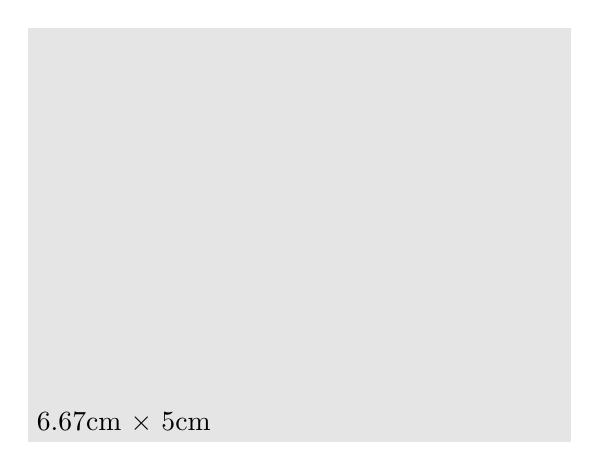
\begin{tikzpicture}
    \node [text width=6.67cm, text height=5cm, fill=gray!20] {6.67cm $\times$ 5cm};    
  \end{tikzpicture}
  \caption{单幅插图示例\label{fig:ex1}}  
\end{figure}

一幅图如有若干幅分图,均应编分图号,用(a),(b),(c),... 按顺序编排,且各分图的分题注直
接列在各自分图的正下方,总题注列在所有分图的下方正中,如图\ref{fig:ex2}所示。

\begin{figure}[!ht]
  \centering
  \subcaptionbox{分图示例\label{fig:ex2a}}{\tikz\node[text width=4cm, text height=3cm, fill=red!20]{};}
  \subcaptionbox{分图示例\label{fig:ex2b}}{\tikz\node[text width=4cm, text height=3cm, fill=green!20]{};}
  \subcaptionbox{分图示例\label{fig:ex2c}}{\tikz\node[text width=4cm, text height=3cm, fill=blue!20]{};}
  \caption{插图示例\label{fig:ex2}}
\end{figure}

表格,如表\ref{tab:ex1}所示,表格中各物理量及量纲均按国际标准(SI)及国家规定的法定符号和法定计量单
位标注。一律使用三线表,与文字齐宽,顶线和底线线粗 1.5 磅,中线线粗 1 磅。表格必须通栏,即
表格宽度与正文版面平齐。

\begin{table}[!ht]
  \centering\caption{文献类型和标志代码\label{tab:ex1}}\small
  \begin{tblr}{width=\textwidth,colspec={X[c]X[c]X[c]X[c]},hline{1,2,Z}}
    文献类型   & 标志代码 & 文献类型 & 标志代码 \\
    普通图书   & M        & 会议录   & C        \\
    汇编       & G        & 报纸     & N        \\
    期刊       & J        & 学位论文 & D        \\
    报告       & R        & 标准     & S        \\
    专利       & P        & 数据库   & DB       \\
    计算机程序 & CP       & 电子公告 & EB       \\
  \end{tblr}
\end{table}

在三线表中可以加辅助线,以适应较复杂表格的需要,如表\ref{tab:ex2}所示。

\begin{table}[!ht]
  \centering\caption{方弯管内流动最大速度比较\label{tab:ex2}}\small
  \begin{tblr}{width=\textwidth,colspec={cX[c]X[c]X[c]X[c]},hline{1,2,3,Z},%
      cell{1}{1}={r=2}{font=\bfseries},%
      cell{1}{2,4}={c=2}{c},%
    }
    项目&层流&&紊流&\\
    &0\textdegree 截面&90\textdegree 截面&0\textdegree 截面&90\textdegree 截面\\
    理论值\,$V_{max}/m\cdot{}s^{-1}$& 0.04 & 0.03 & 1.30 & 1.25\\
    计算值\,$V_{max}/m\cdot{}s^{-1}$& 0.04 & 0.03 & 1.26 & 1.21\\
    误差/$\%$ & 0.00 & 3.12  & 3.07& 3.20\\
  \end{tblr}  
\end{table}

公式:公式中各物理量及量纲均按国际标准(SI)及国家规定的法定符号和法定计量单位标注,禁止使
用已废弃的符号和计量单位。公式后应注明编号,公式号应置于小括号中,如(2-3)。写在右边行末,中
间不加虚线。例:

\begin{equation}
  \label{eq:1}
  y=ax^3+bx+\frac{c}{x}+d
\end{equation}

\section{毕业论文(设计)文本打印格式要求}

\begin{enumerate}
\item 毕业论文(设计说明书)成文文稿一律采用计算机打印,采用 A4 规格复
  印纸单面输出\footnote{大数据与智能工程学院要求双面打印,但未对原创声
    明、中英文摘要、参考文献、指导教师简介、致谢等特殊页的打印做说明。
    所以,我们按排版惯例处理,即,按常规“章”处理,一律右页起始。},左边留一
  定装订边距,用学校统一封面格式装订。打印时,页面设置为:
  \begin{enumerate}
  \item 上下页边距均为 3cm,左页边距为 2.5cm,右页边距为 2cm,装订边 0.5cm;
  \item 页眉与页脚的边距均为 2cm,奇数页页眉内容为“论文中文题目”,偶数页页眉内容
    为“第 X 章\hspace{1ex}XXX”,如“1\hspace{1ex}前言”,采用宋体小5号字
    居中排写\footnote{每章首页是否要有页眉,学校没说,所以,我们按排版
      惯例处理,即,首页不要页眉。};
  \item 正文字间距为标准,行间距为1.5倍行距,段前段后不空行;
  \item 页码一律位于页面底端(页脚),居中标明。
  \end{enumerate}
\item 毕业论文(设计)文本字体和格式要求
  \begin{enumerate}
  \item 中文题目使用小2号黑体字、居中,署名使用4号宋体字\footnote{显然
      这是在说摘要页题目和署名。封面上的题目该用几号字,没有规范。};中
    文摘要、关键词的内容为5号宋体字,“摘要、关键词”5个字用小4号黑体字;
    英文题目使用3号Times New Roman体、居中;英文摘要、关键词内容使用
    小4号Times New Roman体字;正文统一使用小4号宋体和Times New Roman字
    体;图、表内容使用5号宋体和Times New Roman字体{\bug}\footnote{图片
      中的字号,本来就是有大有小,怎么可能统一用5号?图片字号比正文略小
      就行了。};公式字体、字号与正文相同;
  \item 文本一级标题使用小3号黑体字,二级标题使用4号黑体字,三级标题使用小4号黑体字;
  \item 注释、参考文献使用5号宋体字,“注释、参考文献”六个字用4号黑
    体{\bug}\footnote{第\ref{sec:endnote}节中说,注释要用尾注方式。因为
      是“尾注”,也就是在每章末尾列出注释,所以“注释”二字排版与二级标题
      一致,采用4号黑体字,这是没问题的。但第\ref{sec:endnote}节中也说
      到,参考文献要列于论文的最后,也就是说,不是以尾注的形式出现,而
      是以独立一章的形式出现,故“参考文献”四字显然应以章标题形式出现,
      用小3号黑体字。}。
  \end{enumerate}
\end{enumerate}

\section{毕业论文(设计)文本装订规范}

\begin{enumerate}
\item 毕业论文(设计)文本按如下次序装订成册。
  \begin{enumerate}
  \item 封面;
  \item 原创性声明;
  \item 中文摘要及关键词;
  \item 英文摘要及关键词;
  \item 目录;
  \item 正文;
  \item 参考文献;
  \item 指导教师简介;
  \item 致谢;
  \item 附录(必要时可加此部分,如程序清单等);
  \item 封底。
  \end{enumerate}
\item 附件另行装订。毕业论文(设计)材料较多,且不宜收入正文中的有关材料,如译文及原文、专
  题调研报告、过长的公式推演过程、非软件设计题目中篇幅较大的计算机程序等,可按如下次序装订
  成册:
  \begin{enumerate}
  \item 封面;
  \item 目录;
  \item 调研报告、文献综述;
  \item 外文翻译及原文(译文在前,原文在后);
  \item 公式推演过程、计算机程序等;
  \item 封底。
  \end{enumerate}
\item 某些特殊专业毕业论文(设计)文本、图纸等较多时,应按要求整理完毕后装入专用资料袋,其
  封面要用仿宋字认真填写,做到资料齐全、工整美观;
\item 毕业论文(设计)任务书、毕业论文(设计)实习计划表、毕业论文(设计)开题报告、毕业论
  文(设计)中期检查表、毕业论文(设计)答辩记录表、毕业论文(设计)指导教师意见、毕业论文
  (设计)评阅意见、查重检测报告、毕业论文(设计)、答辩评分表及其它归档材料一并装入“西南林
  业大学大学毕业论文(设计)档案袋”,由学生所在学院归档保管。
\end{enumerate}

\section{其他要求}

专科学生毕业论文(设计)撰写规范参照本科执行。相关表格可到教务处网页下载。

%%% Local Variables:
%%% mode: LaTeX
%%% TeX-master: "../tutorial"
%%% End:
